\subsection{Recorded selection changes}\label{app:selection-changes}

The observer in \cref{fig:fw-selection-changes} refuses changed evaluation
identities, inconsistent selection counts and duplicate context identifiers
before comparing ordered program identities. It counts candidate and retained
differences from one stored reference, rather than utility changes.
The tie-admission and best-round identity rules follow
\cref{sec:method-status}.
These changes occur on reused development contexts; matched controls are
still required for \mbox{attribution to training} or proposal quality.

\begin{figure}[htbp]
  \centering
  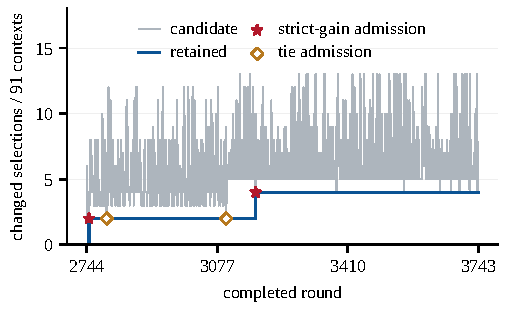
\includegraphics[width=\linewidth]{figures/fig_fw_selection_changes.pdf}
  \caption{\textbf{Retained program selections change only at admitted rounds.}
  Rounds 2744--3743, captured at 14:34 UTC on 2 November 2026.
  All \num{1000} completed records compare selections on 91 reused
  development contexts with the recorded round-882 reference.
  Grey: candidate before admission; blue: post-decision retained selections.
  Stars: two strict-gain admissions; hollow diamonds: two accepted ties;
  the other 996 decisions are rejections. These descriptive identity
  counts do not establish a training effect, writer or ranking-map benefit,
  or independent proposal quality. Scope: \cref{sec:method-status}.}
  \label{fig:fw-selection-changes}
\end{figure}
